Důležitou částí této práce je aplikace, která umožňuje pro konkrétní vstupní data vypočítat výnosy fotovoltaické elektrárny a výpočet různých investičních metrik.
Nejdříve je popsána použitá technologie a zdroje dat, následně jsou uvedeny konkrétní příklady výpočtů.

\section{Popis aplikace}

Veškerá implementace byla provedena v programovacím jazyce Python. Python je moderní programovací jazyk, který je využívaný v mnoha oblastech, například v analýze dat, strojovém učení nebo vývoji webových aplikací.



\subsection{Použité technologie}

\subsubsection{FastAPI} je moderní webový framework pro tvorbu REST API.
Jiným, též populárním frameworkem pro tvorbu REST API je Flask.

\subsubsection{PuLP} je knihovna pro lineární programování.
Alternativami ke knihovně PuLP jsou například CVXOPT nebo SciPy.

\subsubsection{InfluxDB} je open-source databáze optimalizovaná pro časové řady.
Jiné databáze určené pro časové řady jsou například TimescaleDB nebo Prometheus.

\subsection{Data}

Pro výpočet výnosů fotovoltaických elektráren byla použita data z několika zdrojů.

\subsubsection*{OTE, a.s.}
(Operátor trhu s elektřinou) je akciová společnost, která funguje jako operátor trhu s energiemi.
Má na starosti organizování krátkodobého trhu s elektřinou a plynem.
% https://www.ote-cr.cz/cs/o-spolecnosti/zpravy_ote/objemy-energii-zobchodovanych-na-kratkodobych-trzich-s-elektrinou-a-plynem-ote-trvale-rostou
\begin{figure}[H]
    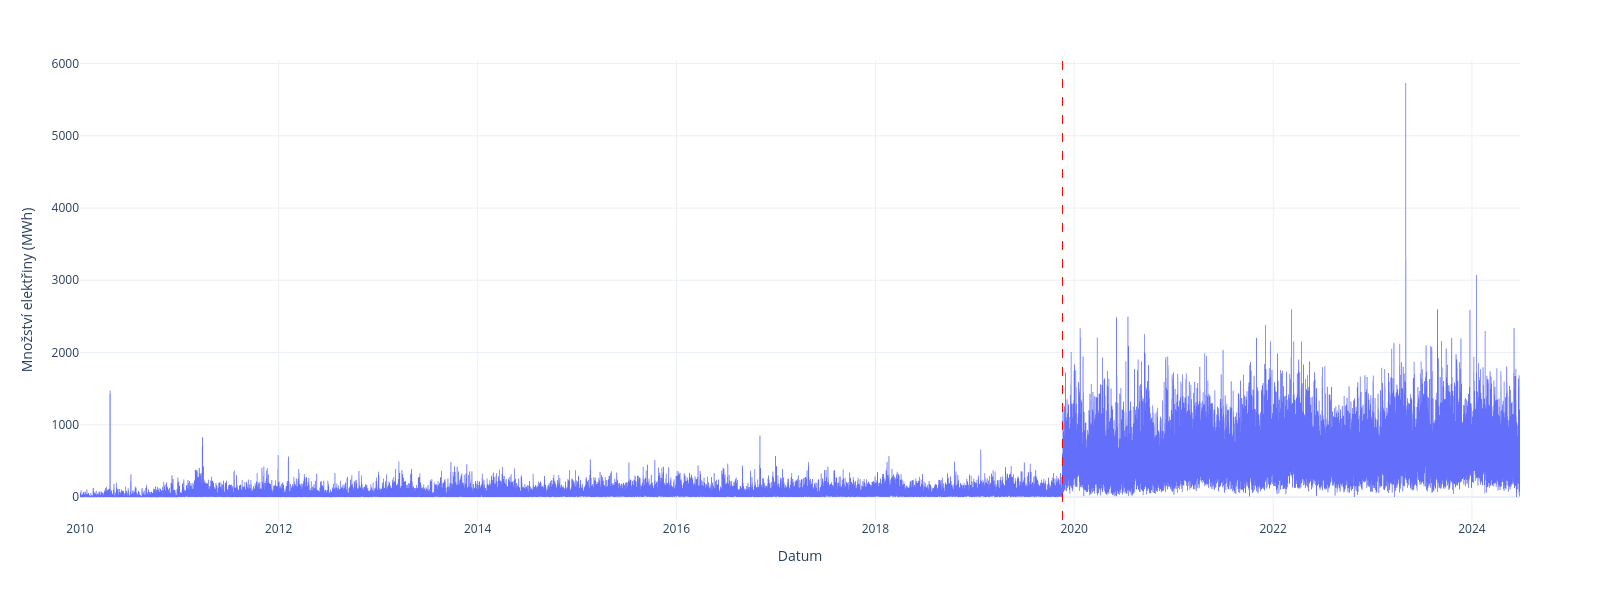
\includegraphics[width=\textwidth]{static/graphs/ote.png}
    \caption{Zobchodované množství elektřiny 2010--2024}
    \label{fig:ote}
\end{figure}

 
\subsubsection*{ČHMÚ} (Český hydrometeorologický ústav) musí zpřístupnit denní, měsiční a roční klimatologické charakteristiky za období 1961--2023. \footnote[1]{Zákon č. 123/1998 Sb., o právu na informace o životním prostředí.}

Denní úhrn doby trvání slunečního svitu je časový interval mezi východem a západem Slunce,
během kterého není sluneční kotouč zakrytý oblačností nebo jinými překážkami.
Fyzikálně je definován jako doba, kdy je intenzita toku přímého slunečního záření vyšší než 120 \si{\watt}/\si{\meter\squared}.
Udává se v hodinách.

\href{https://www.chmi.cz/files/portal/docs/meteo/ok/open_data_2023/Podminky_uziti_udaju.pdf}{Podmínky užití dat}

\begin{figure}[H]
    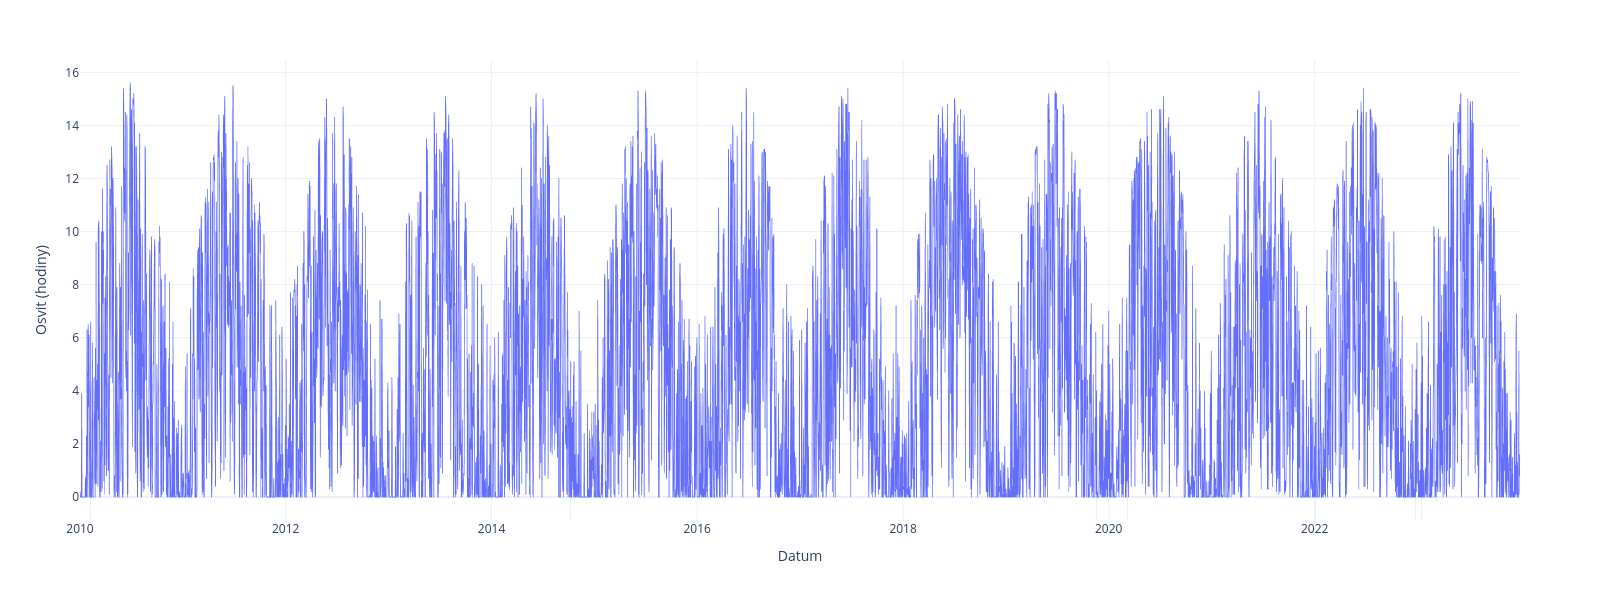
\includegraphics[width=\textwidth]{static/graphs/osvit.png}
    \caption{ČHMÚ. Osvitové hodiny 2010--2023}
    \label{fig:ote}
\end{figure}


\section{Konkrétní příklady}